% 2007 年四川卷理科第 14 题：正三棱柱 ABC-A_1B_1C_1 及直线 BC_1。
% 来源 PDF：gaokaomath-src/普通高考/2007/2007四川理.pdf，SHA256 6f3287a6ec1c136fb7e457cb0264d069c44eb8ff58a81cc3598f9c8f1395cc2d
% 原页：2007四川理.pdf 第 1 页（A3 三栏）第 3 栏，书页码 409，图在第 14 题题干下方。
% 重绘依据：竖放正三棱柱的斜二测画法，上底 A_1B_1C_1 中 A_1 在左、B_1 在右、
%   C_1 在后上方（自 A_1B_1 中点沿 45° 纵深方向偏移）；侧棱竖直，侧棱长与底面边长
%   之比按题设 √2:1 = 1.41 取（底面边长 2、高 2.83）。上底三边、可见侧棱 A_1A、B_1B
%   与可见底边 AB 画实线；不可见的底边 AC、CB、侧棱 CC_1 与辅助线 BC_1 画虚线。
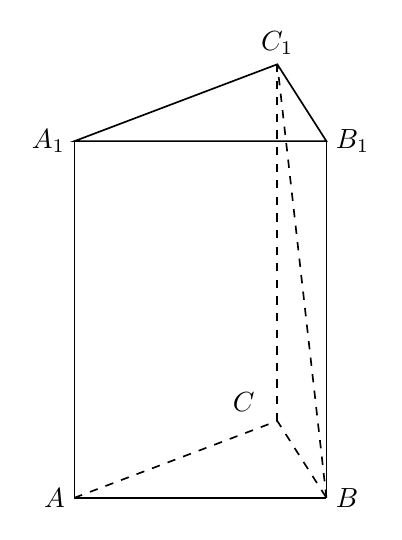
\begin{tikzpicture}[scale=1.6, semithick,
  every node/.style={inner sep=1.5pt}]
  \coordinate (A1) at (0,0);
  \coordinate (B1) at (2,0);
  \coordinate (C1) at (1.61,0.61);
  \coordinate (A)  at (0,-2.83);
  \coordinate (B)  at (2,-2.83);
  \coordinate (C)  at (1.61,-2.22);
  % 不可见的三条棱与辅助线
  \draw[dashed] (A) -- (C) -- (B);
  \draw[dashed] (C) -- (C1);
  \draw[dashed] (B) -- (C1);
  % 可见的侧棱与底边
  \draw (A1) -- (A);
  \draw (B1) -- (B);
  \draw (A) -- (B);
  % 上底
  \draw (A1) -- (B1) -- (C1) -- cycle;
  \node[anchor=east] at ([xshift=-1pt]A1) {$A_1$};
  \node[anchor=west] at ([xshift=1pt]B1) {$B_1$};
  \node[anchor=south] at ([yshift=1pt]C1) {$C_1$};
  \node[anchor=east] at ([xshift=-1pt]A) {$A$};
  \node[anchor=west] at ([xshift=1pt]B) {$B$};
  \node[anchor=south east] at ([xshift=-4pt,yshift=1pt]C) {$C$};
\end{tikzpicture}
